%%%%%%%%%%%%%%%%%%%%%%%%%%%%%%%%%%%%%%%%%%%%%%%%%%%%%%%%%%%%%%%%%%%%%%%%%%%%%%%%%%
\begin{frame}[fragile]\frametitle{}
\begin{center}
{\Large Functions}
\end{center}
\end{frame}


%%%%%%%%%%%%%%%%%%%%%%%%%%%%%%%%%%%%%%%%%%%%%%%%%%%%%%%%%%%%%%%%%%%%%%%%%%%%%%%%%%%
\begin{frame}[fragile]\frametitle{Function calls}
    \begin{itemize}
    \item  A function is a named sequence of statements that
performs a computation. 
    \item  When you define a function, you specify the name and
the sequence of statements. 
    \item  Later, you can ``call'' the function by name.
    \end{itemize}
\begin{lstlisting}
>>> type(32)
<class 'int'>
\end{lstlisting}
    \begin{itemize}
    \item  The name of the function is type. 
    \item The expression in parentheses is called the argument of the function. 
    \item The argument is a value or variable that we are passing into the function as input to the function.
    \item The result, for the type function, is the type of the argument.
    \end{itemize}
\end{frame}

%%%%%%%%%%%%%%%%%%%%%%%%%%%%%%%%%%%%%%%%%%%%%%%%%%%%%%%%%%%%%%%%%%%%%%%%%%%%%%%%%%%
\begin{frame}[fragile]\frametitle{Built-in functions}
Python provides a set of functions already built-in. You are already very familiar with one of them:
\begin{lstlisting}
print(''Oh yeah, I am a function!\n'')

name = input(''I get inputs from you! What is your name?'')
print(''Hello'', name)

nums = [3, 41, 12, 9, 74, 15]
print(''Length:'', len(nums))
print(''Max:'', max(nums))
print(''Min:'', min(nums))
print(''Sum:'', sum(nums))

list(range(-10,10,2))

a = [0.819, 0.277, 0.817, 0.575, 0.168, 0.973, 0.987, 0.883, 0.293, 0.933]
# Keep only numbers above 0.5 and round them to 2 decimals
b = [round(num,2) for num in a if num>0.5]
print(sorted(b))
\end{lstlisting}
\end{frame}


%%%%%%%%%%%%%%%%%%%%%%%%%%%%%%%%%%%%%%%%%%%%%%%%%%%%%%%%%%%%%%%%%%%%%%%%%%%%%%%%%%%
\begin{frame}[fragile]\frametitle{Functions from Libraries}
We can also add more functions by import-ing libraries, like the math library. 
\begin{lstlisting}
# Let's have some fun
import math
for i in range(32):
    # math.fabs returns the absolute value
    # math.cos returns the cosine of the value
    x = int(math.fabs((i*math.cos(i/4)))+1)
    print(x*'#')
    
import random
for i in range(10):
    x = random.random()
    print(round(x,3))
\end{lstlisting}
\end{frame}


%%%%%%%%%%%%%%%%%%%%%%%%%%%%%%%%%%%%%%%%%%%%%%%%%%%%%%%%%%%%%%%%%%%%%%%%%%%%%%%%%%%
\begin{frame}[fragile]\frametitle{User Defined Functions}
A function in Python is defined by a def statement. The general syntax looks like this:
\begin{lstlisting}
def function-name(Parameter list):
    statements, i.e. the function body
\end{lstlisting}
    \begin{itemize}
    \item  The parameter list consists of none or more parameters. 
    \item Parameters are called arguments, if the function is called.
    \item The function body consists of indented statements. 
    \item The function body gets executed every time the function is called. 
    \end{itemize}
\end{frame}

%%%%%%%%%%%%%%%%%%%%%%%%%%%%%%%%%%%%%%%%%%%%%%%%%%%%%%%%%%%%%%%%%%%%%%%%%%%%%%%%%%%%%
%%\begin{frame}[fragile]\frametitle{How to define new functions}
%%\begin{lstlisting}
%%def greet(name):
%%  ''''''
%%  A friendly function.
%%  ''''''
%%  print (''Hello, '' + name + ''!'')
%%
%%# the customary greeting
%%greet(''world'')
%%\end{lstlisting}
%%\end{frame}



%%%%%%%%%%%%%%%%%%%%%%%%%%%%%%%%%%%%%%%%%%%%%%%%%%%%%%%%%%%%%%%%%%%%%%%%%%%%%%%%%%%
\begin{frame}[fragile]\frametitle{User Defined Functions}
Functions assign a name to a block of code the way variables assign names to bits of data.
\begin{lstlisting}
def print_hi():
    print(''hi!'')

for i in range(10):
    print_hi()
    
def hi_you(name):
    print(''HI {n}!''.format(n=name.upper()))
    
hi_you(''David'')
\end{lstlisting}
\end{frame}

%%%%%%%%%%%%%%%%%%%%%%%%%%%%%%%%%%%%%%%%%%%%%%%%%%%%%%%%%%%%%%%%%%%%%%%%%%%%%%%%%%%
\begin{frame}[fragile]\frametitle{The `return' statement }
    \begin{itemize}
    \item  Function bodies can contain one or more return statement. 
    \item They can be situated anywhere in the function body. 
    \item A return statement ends the execution of the function call and ''returns'' the result, i.e. the value of the expression following the return keyword, to the caller. 
    \item If the return statement is without an expression, the special value None is returned.
    \item If there is no return statement in the function code, the function ends, when the control flow reaches the end of the function body and the value ''None'' will be returned. 
    \end{itemize}
\end{frame}



%%%%%%%%%%%%%%%%%%%%%%%%%%%%%%%%%%%%%%%%%%%%%%%%%%%%%%%%%%%%%%%%%%%%%%%%%%%%%%%%%%%
\begin{frame}[fragile]\frametitle{The `return' statement }
Example of computing a math function:
\begin{lstlisting}
def square(num):
    squared = num*num
    return squared

x = square(123232)
print(x)

for i in range(15):
    print(''The square of {a} is {aa}''.format(a=i, aa=square(i)))
\end{lstlisting}
\end{frame}

%%%%%%%%%%%%%%%%%%%%%%%%%%%%%%%%%%%%%%%%%%%%%%%%%%%%%%%%%%%%%%%%%%%%%%%%%%%%%%%%%%%
\begin{frame}[fragile]\frametitle{Returning Multiple Values}
    \begin{itemize}
    \item  A function can return exactly one value, or we should better say one object. 
    \item An object can be a numerical value, like an integer or a float. 
    \item But it can also be e.g. a list or a dictionary. 
    \item So, if we have to return for example 3 integer values, we can return a list or a tuple with these three integer values. 
    \item This means that we can indirectly return multiple values.
    \item If only ``,'' are seen, thats actually a tuple.
        \end{itemize}
\end{frame}

%%%%%%%%%%%%%%%%%%%%%%%%%%%%%%%%%%%%%%%%%%%%%%%%%%%%%%%%%%%%%%%%%%%%%%%%%%%%%%%%%%%
\begin{frame}[fragile]\frametitle{Exercises}
    \begin{itemize}
    \item  Write a function `in\_range' that checks if a number `n' is within a given range `(a,b)' and returns True or False. 
    \item The function takes n, a, and b as parameters.
%    \item Write a dedup function that takes as input a list and returns back another list, with only unique elements and sorted. For example, if the input is [1,2,5,5,5,3,3,3,3,4,5] the returned list should be [1, 2, 3, 4, 5]. If the input is ['New York', 'New York',  'Paris', 'London', 'Paris'] the returned list should be ['London', 'New York', 'Paris'].
%    \item Write a function that generates a random password with n letters. The value n should be a parameter.
%    \begin{lstlisting}
%# This code generates one random letter
%import random
%import string
%random.choice(string.ascii_letters)
%\end{lstlisting}
    \end{itemize}
\end{frame}

%%%%%%%%%%%%%%%%%%%%%%%%%%%%%%%%%%%%%%%%%%%%%%%%%%%%%%%%%%%%%%%%%%%%%%%%%%%%%%%%%%%
\begin{frame}[fragile]\frametitle{Exercise}
\begin{itemize}
\item Insert at least two distinct functions.
\item Factorial
\item Fibonacci
\end{itemize}
\end{frame}

% %%%%%%%%%%%%%%%%%%%%%%%%%%%%%%%%%%%%%%%%%%%%%%%%%%%%%%%%%%%%%%%%%%%%%%%%%%%%%%%%%%%
% \begin{frame}[fragile]\frametitle{Exercise}
  % \begin{itemize}
  % \item Write a program which can compute the factorial of a given numbers.
  % \item The results should be printed in a comma-separated sequence on a single line.
  % \item Suppose the following input is supplied to the program:8
  % \item Then, the output should be:40320
  % \end{itemize}  
% \end{frame}

%%%%%%%%%%%%%%%%%%%%%%%%%%%%%%%%%%%%%%%%%%%%%%%%%%%%%%%%%%%%%%%%%%%%%%%%%%%%%%%%%%%
\begin{frame}[fragile]\frametitle{Solution}
Factorial
  \begin{lstlisting}
def fact(x):
    if x == 0:
        return 1
    return x * fact(x - 1)

x=int(input())
print(fact(x))
  \end{lstlisting}
\end{frame}

%%%%%%%%%%%%%%%%%%%%%%%%%%%%%%%%%%%%%%%%%%%%%%%%%%%%%%%%%%%%%%%%%%%%%%%%%%%%%%%%%%%
\begin{frame}[fragile]\frametitle{Solutions}
Fibonacci
\begin{lstlisting}
    def fibonacci(n):
        if n == 0: 
            return 1
        elif n == 1: 
            return 1
        else: 
            return fibonacci(n-1)+ fibonacci(n-2)
\end{lstlisting}
\end{frame}


%%%%%%%%%%%%%%%%%%%%%%%%%%%%%%%%%%%%%%%%%%%%%%%%%%%%%%%%%%%%%%%%%%%%%%%%%%%%%%%%%%%
\begin{frame}[fragile]\frametitle{Exercise}
Please write a program to shuffle and print the list [3,6,7,8].

Hints:
Use random.shuffle() function to shuffle a list.
\end{frame}

%%%%%%%%%%%%%%%%%%%%%%%%%%%%%%%%%%%%%%%%%%%%%%%%%%%%%%%%%%%%%%%%%%%%%%%%%%%%%%%%%%%
\begin{frame}[fragile]\frametitle{Solution}
\begin{lstlisting}
from random import shuffle
li = [3,6,7,8]
shuffle(li)
print(li)
\end{lstlisting}
\end{frame}


%%%%%%%%%%%%%%%%%%%%%%%%%%%%%%%%%%%%%%%%%%%%%%%%%%%%%%%%%%%%%%%%%%%%%%%%%%%%%%%%%%%
\begin{frame}[fragile]\frametitle{Exercise}
    \begin{itemize}
    \item  Please write a binary search function which searches an item in a sorted list.
    \item The function should return the index of element to be searched in the list.
    \item Hints: Use if/elif to deal with conditions.
    \end{itemize}
\end{frame}

%%%%%%%%%%%%%%%%%%%%%%%%%%%%%%%%%%%%%%%%%%%%%%%%%%%%%%%%%%%%%%%%%%%%%%%%%%%%%%%%%%%
\begin{frame}[fragile]\frametitle{Solution}
\begin{lstlisting}
import math
def bin_search(li, element):
    bottom = 0
    top = len(li)-1
    index = -1
    while top>=bottom and index==-1:
        mid = int(math.floor((top+bottom)/2.0))
        if li[mid]==element:
            index = mid
        elif li[mid]>element:
            top = mid-1
        else:
            bottom = mid+1

    return index

li=[2,5,7,9,11,17,222]
print(bin_search(li,11))
print(bin_search(li,12))
\end{lstlisting}
\end{frame}

%%%%%%%%%%%%%%%%%%%%%%%%%%%%%%%%%%%%%%%%%%%%%%%%%%%%%%%%%%%%%%%%%%%%%%%%%%%%%%%%%%%
\begin{frame}[fragile]\frametitle{Example function: Cleaning up a string}
\begin{lstlisting}
def clean(phone):
    result = ''''
    digits = {''0'',''1'',''2'',''3'',''4'',''5'',''6'',''7'',''8'',''9''}
    for c in phone:
        if c in digits:
            result = result + c
    return result        
    
p = ''(800) 555-1214 Panos Phone number''
print(clean(p))
\end{lstlisting}
Output??
\end{frame}

%
%%%%%%%%%%%%%%%%%%%%%%%%%%%%%%%%%%%%%%%%%%%%%%%%%%%%%%%%%%%%%%%%%%%%%%%%%%%%%%%%%%%%
%\begin{frame}[fragile]\frametitle{Functions, I}
%Casts are also functions.
%\begin{lstlisting}
%>>> int(''42'')
%42
%>>> int(4.2)
%4
%>>> float(42)
%42.0
%>>> str(42)
%'42'
%>>> str()
%''
%\end{lstlisting}
%\end{frame}

%%%%%%%%%%%%%%%%%%%%%%%%%%%%%%%%%%%%%%%%%%%%%%%%%%%%%%%%%%%%%%%%%%%%%%%%%%%%%%%%%%%
\begin{frame}[fragile]\frametitle{Exercise}
  \begin{itemize}
  \item Write a program that computes the value of a+aa+aaa+aaaa with a given digit as the value of a.
  \item Suppose the following input is supplied to the program: 9
  \item Then, the output should be: 11106
  \item Hints: int cast on tuple of numbers, yields the number

  \end{itemize}  
\end{frame}

%%%%%%%%%%%%%%%%%%%%%%%%%%%%%%%%%%%%%%%%%%%%%%%%%%%%%%%%%%%%%%%%%%%%%%%%%%%%%%%%%%%
\begin{frame}[fragile]\frametitle{Solution}
  \begin{lstlisting}
a = input()
n1 = int("{}".format(a))
n2 = int("{}{}".format(a,a) )
n3 = int("{}{}{}".format(a,a,a) )
n4 = int("{}{}{}{}".format(a,a,a,a) )
print(n1+n2+n3+n4)
  \end{lstlisting}
\end{frame}



%%%%%%%%%%%%%%%%%%%%%%%%%%%%%%%%%%%%%%%%%%%%%%%%%%%%%%%%%%%%%%%%%%%%%%%%%%%%%%%%%%%
\begin{frame}[fragile]\frametitle{Variable number of arguments}
  Some functions can take a variable number of arguments:
  \begin{itemize}
    \item {\bf sum([$x_0$, \ldots, $x_n$])} Return $x_0 + \cdots + x_n$.
    \item{\bf max($x_0$, \ldots, $x_n$)} Return the maximum of the set $\{ x_0, \ldots, x_n \}$
    \item {\bf min($x_0$, \ldots, $x_n$)} Return the minimum of the set $\{ x_0, \ldots, x_n \}$
  \end{itemize}

  
  Examples:
\begin{lstlisting}
>>> sum([1,2,3])
6
>>> min(1,2,3)
1
>>> max(1,2)
2
\end{lstlisting}

\end{frame}

%%%%%%%%%%%%%%%%%%%%%%%%%%%%%%%%%%%%%%%%%%%%%%%%%%%%%%%%%%%%%%%%%%%%%%%%%%%%%%%%%%%
\begin{frame}[fragile]\frametitle{The most important function of all}
{\bf help(\texttt{fn})} Display help on the function named \texttt{fn}
What happens if you type these at the prompt?
    \begin{itemize}
    \item \texttt{help(abs)}
    \item \texttt{help(max)}
    \end{itemize}
Without any argument, \texttt{help()}: starts an interactive help prompt.
\begin{lstlisting}
 >>> help()
\end{lstlisting}
\end{frame}


%%%%%%%%%%%%%%%%%%%%%%%%%%%%%%%%%%%%%%%%%%%%%%%%%%%%%%%%%%%%%%%%%%%%%%%%%%%%%%%%%%%%%
%%\begin{frame}[fragile]\frametitle{Answer}
%%What is this? The answer in the next exercise!
%%\begin{lstlisting}
%%def greet(name):
%%  ''''''
%%  A friendly function.
%%  ''''''
%%  print (''Hello, '' + name + ''!'')
%%
%%# the customary greeting
%%greet(''world'')
%%\end{lstlisting}
%%\end{frame}

%%%%%%%%%%%%%%%%%%%%%%%%%%%%%%%%%%%%%%%%%%%%%%%%%%%%%%%%%%%%%%%%%%%%%%%%%%%%%%%%%%%
\begin{frame}[fragile]\frametitle{Default values}

  Function arguments can have default values.
\begin{lstlisting}
>>> def hello(name='world'):
...   print (''Hello, '' + name)
...
>>> hello()
'Hello, world'
\end{lstlisting}
\end{frame}

%%%%%%%%%%%%%%%%%%%%%%%%%%%%%%%%%%%%%%%%%%%%%%%%%%%%%%%%%%%%%%%%%%%%%%%%%%%%%%%%%%%
\begin{frame}[fragile]\frametitle{Named arguments}
Python allows calling a function with named arguments:
\begin{lstlisting}
hello(name=''Alice'')
\end{lstlisting}
When passing arguments by name, they can be passed in any order:
\begin{lstlisting}
>>> from fractions import Fraction
>>> Fraction(numerator=1, denominator=2)
Fraction(1, 2)
>>> Fraction(denominator=2, numerator=1)
Fraction(1, 2)
\end{lstlisting}
\end{frame}


%%%%%%%%%%%%%%%%%%%%%%%%%%%%%%%%%%%%%%%%%%%%%%%%%%%%%%%%%%%%%%%%%%%%%%%%%%%%%%%%%%%
\begin{frame}[fragile]\frametitle{Variable Scope Rules}
Whatever happens in a function stays in a function
    \begin{itemize}
    \item Variables set inside of functions are scoped to those functions: changes, including any new variables created, are only accessible inside in the function.
    \item If ``outside'' variables are modified inside a function's context, the contents of that variable are first copied.
	\item Similarly, changes or modifications to a function's arguments aren't reflected once the scope is returned; The variable will continue to point to the original thing. 
	\item However, it is possible to modify the thing that is passed, assuming that it is mutable.
    \end{itemize}
\end{frame}

%%%%%%%%%%%%%%%%%%%%%%%%%%%%%%%%%%%%%%%%%%%%%%%%%%%%%%%%%%%%%%%%%%%%%%%%%%%%%%%%%%%
\begin{frame}[fragile]\frametitle{Variable Scope}
Whatever happens in a function stays in a function
\begin{lstlisting}
def times_two(inp):
    inp = 2*inp
    return inp

variable_four = 4
print(times_two(variable_four))
print(variable_four)
\end{lstlisting}
\end{frame}


%%%%%%%%%%%%%%%%%%%%%%%%%%%%%%%%%%%%%%%%%%%%%%%%%%%%%%%%%%%%%%%%%%%%%%%%%%%%%%%%%%%
\begin{frame}[fragile]\frametitle{Variable Scope}
\begin{lstlisting}
def f(): 
    print(s) 
s = ''I love Paris in the summer!''
f()
\end{lstlisting}

    \begin{itemize}
    \item The variable s is defined as the string ''I love Paris in the summer!'', before calling the function f(). 
    \item The body of f() consists solely of the ''print(s)'' statement. 
    \item As there is no local variable s, i.e. no assignment to s, the value from the global variable s will be used. 
    \item So the output will be the string ''I love Paris in the summer!''.
    \end{itemize}
\end{frame}

%%%%%%%%%%%%%%%%%%%%%%%%%%%%%%%%%%%%%%%%%%%%%%%%%%%%%%%%%%%%%%%%%%%%%%%%%%%%%%%%%%%
\begin{frame}[fragile]\frametitle{Variable Scope}

    \begin{itemize}
    \item What will happen, if we change the value of s inside of the function f()?
    \item  Will it affect the global variable as well?
    \end{itemize}
\begin{lstlisting}
def f(): 
    s = ''I love London!''
    print(s) 

s = ''I love Paris!'' 
f()
print(s)

I love London!
I love Paris!
\end{lstlisting}

\end{frame}

%%%%%%%%%%%%%%%%%%%%%%%%%%%%%%%%%%%%%%%%%%%%%%%%%%%%%%%%%%%%%%%%%%%%%%%%%%%%%%%%%%%
\begin{frame}[fragile]\frametitle{Variable Scope}
\begin{lstlisting}
name = ''panos''
def do_something():
    print(''We are now in the function!'')
    name = ''not panos''
    print(name)
    print(''something! ... and we are out'')
    
print(''We start here!'')
print(''The name is'', name)
print(''Let's call the function...'')
do_something()
print(''Done with the function...'')
print(name)
\end{lstlisting}
\end{frame}

%%%%%%%%%%%%%%%%%%%%%%%%%%%%%%%%%%%%%%%%%%%%%%%%%%%%%%%%%%%%%%%%%%%%%%%%%%%%%%%%%%%
\begin{frame}[fragile]\frametitle{Variable Scope}

    \begin{itemize}
    \item What if we combine the first example with the second one, i.e. we first access s with a print() function, hoping to get the global value, and then assigning a new value to it? 
    \item Assigning a value to it, means - as we have previously stated - creating a local variable s. 
    \item So, we would have s both as a global and a local variable in the same scope, i.e. the body of the function. 
    \item Python fortunately doesn't allow this ambiguity. So, it will throw an error
    \end{itemize}
\begin{lstlisting}
>>> def f(): 
...   print(s)
...   s = ''I love London!''
...   print(s)
... 
>>> s = ''I love Paris!''
>>> f()
Traceback (most recent call last):
  File ''<stdin>'', line 1, in <module>
  File ''<stdin>'', line 2, in f
UnboundLocalError: local variable 's' referenced before assignment
>>> 
\end{lstlisting}

\end{frame}

%%%%%%%%%%%%%%%%%%%%%%%%%%%%%%%%%%%%%%%%%%%%%%%%%%%%%%%%%%%%%%%%%%%%%%%%%%%%%%%%%%%
\begin{frame}[fragile]\frametitle{Variable Scope}

    \begin{itemize}
    \item A variable can't be both local and global inside of a function. 
    	\item So Python decides that we want a local variable due to the assignment to s inside of f(), so the first print statement before the definition of s throws the error message above.
    	\item Any variable which is changed or created inside of a function is local, if it hasn't been declared as a global variable. 
    	\item To tell Python, that we want to use the global variable, we have to explicitly state this by using the keyword ''global''
    \end{itemize}

\end{frame}

%%%%%%%%%%%%%%%%%%%%%%%%%%%%%%%%%%%%%%%%%%%%%%%%%%%%%%%%%%%%%%%%%%%%%%%%%%%%%%%%%%%
\begin{frame}[fragile]\frametitle{Variable Scope}

\begin{lstlisting}
def f():
    global s
    print(s)
    s = ''Only in spring, but London is great as well!''
    print(s)

s = ''I am looking for a course in Paris!'' 
f()
print(s)

I am looking for a course in Paris!
Only in spring, but London is great as well!
Only in spring, but London is great as well!
\end{lstlisting}

\end{frame}

%%%%%%%%%%%%%%%%%%%%%%%%%%%%%%%%%%%%%%%%%%%%%%%%%%%%%%%%%%%%%%%%%%%%%%%%%%%%%%%%%%%
\begin{frame}[fragile]\frametitle{Variable Scope}
Local variables of functions can't be accessed from outside, when the function call has finished:
\begin{lstlisting}
def f():
    s = ''I am globally not known''
    print(s) 

f()
print(s)


I am globally not known
Traceback (most recent call last):
  File ''ex.py'', line 6, in <module>
    print(s)
NameError: name 's' is not defined
\end{lstlisting}
\end{frame}


%%%%%%%%%%%%%%%%%%%%%%%%%%%%%%%%%%%%%%%%%%%%%%%%%%%%%%%%%%%%%%%%%%%%%%%%%%%%%%%%%%%
\begin{frame}[fragile]\frametitle{Variable Scope}
The following example shows a wild combination of local and global variables and function parameters:
\begin{lstlisting}
def foo(x, y):
    global a
    a = 42
    x,y = y,x
    b = 33
    b = 17
    c = 100
    print(a,b,x,y)

a, b, x, y = 1, 15, 3,4 
foo(17, 4)
print(a, b, x, y)

42 17 4 17
42 15 3 4
\end{lstlisting}
\end{frame}



%%%%%%%%%%%%%%%%%%%%%%%%%%%%%%%%%%%%%%%%%%%%%%%%%%%%%%%%%%%%%%%%%%%%%%%%%%%%%%%%%%%
\begin{frame}[fragile]\frametitle{Variable Scope}
\begin{lstlisting}
# composite data structures (lists, sets, dictionaries) _can_ be modified
def add_sum(parameter_list):
    s = sum(parameter_list)
    parameter_list.append(s)
    return s

a_list = [1,2,3]
total = add_sum(a_list)
print(total)
print(a_list)

# try again!
tot = add_sum(a_list)
print(tot)
print(a_list)

\end{lstlisting}
\end{frame}


%%%%%%%%%%%%%%%%%%%%%%%%%%%%%%%%%%%%%%%%%%%%%%%%%%%%%%%%%%%%%%%%%%%%%%%%%%%%%%%%%%%
\begin{frame}[fragile]\frametitle{Variable Scope}
\begin{lstlisting}
def append_to_sequence (myseq):
    myseq += (9,9,9)
    return myseq

tuple1 = (1,2,3) # tuples are immutable
list1 = [1,2,3] # lists are mutable

tuple2 = append_to_sequence(tuple1)
list2 = append_to_sequence(list1)

print 'tuple1 = ', tuple1 # outputs (1, 2, 3)
print 'tuple2 = ', tuple2 # outputs (1, 2, 3, 9, 9, 9)
print 'list1 = ', list1 # outputs [1, 2, 3, 9, 9, 9]
print 'list2 = ', list2 # outputs [1, 2, 3, 9, 9, 9]
\end{lstlisting}
  
\end{frame}

%%%%%%%%%%%%%%%%%%%%%%%%%%%%%%%%%%%%%%%%%%%%%%%%%%%%%%%%%%%%%%%%%%%%%%%%%%%%%%%%%%%
\begin{frame}[fragile]\frametitle{Variable Scope}
       \begin{itemize}
    \item  myseq is a local variable of the append\_to\_sequence function, but when this function gets called, myseq will nevertheless point to the same object as the variable that we pass in (t or l in our example).
    \item If that object is immutable (like a tuple), there is no problem. The += operator will cause the creation of a new tuple, and myseq will be set to point to it. 
    \item However, if we pass in a reference to a mutable object, that object will be manipulated in place (so myseq and l, in our case, end up pointing to the same list object).
                \end{itemize}

\end{frame}


%%%%%%%%%%%%%%%%%%%%%%%%%%%%%%%%%%%%%%%%%%%%%%%%%%%%%%%%%%%%%%%%%%%%%%%%%%%%%%%%%%%
\begin{frame}[fragile]\frametitle{Parameters and Arguments}
    \begin{itemize}
    \item Very often the terms parameter and argument are used synonymously, but there is a clear difference. 
        \item Parameters are inside functions or procedures, while arguments are used in procedure calls, i.e. the values passed to the function at run-time. 
            \end{itemize}
\end{frame}

%%%%%%%%%%%%%%%%%%%%%%%%%%%%%%%%%%%%%%%%%%%%%%%%%%%%%%%%%%%%%%%%%%%%%%%%%%%%%%%%%%%
\begin{frame}[fragile]\frametitle{''Call by value'' and ''Call by reference/name''}
    \begin{itemize}
    \item The evaluation strategy for arguments, i.e. how the arguments from a function call are passed to the parameters of the function, differs from programming language to programming language.
    \item The most common evaluation strategies are ''call by value'' and ''call by reference''
            \end{itemize}
\end{frame}

%%%%%%%%%%%%%%%%%%%%%%%%%%%%%%%%%%%%%%%%%%%%%%%%%%%%%%%%%%%%%%%%%%%%%%%%%%%%%%%%%%%
\begin{frame}[fragile]\frametitle{''Call by Value'' }
    \begin{itemize}
    \item Sometimes also called pass-by-value.
    \item Used in C and C++
    \item The argument expression is evaluated, and the result of this evaluation is bound to the corresponding variable in the function. 
    \item So, if the expression is a variable, its value will be assigned (copied) to the corresponding parameter. 
    \item This ensures that the variable in the caller's scope will be unchanged when the function returns. 
            \end{itemize}
\end{frame}

%%%%%%%%%%%%%%%%%%%%%%%%%%%%%%%%%%%%%%%%%%%%%%%%%%%%%%%%%%%%%%%%%%%%%%%%%%%%%%%%%%%
\begin{frame}[fragile]\frametitle{''Call by Reference'' }
    \begin{itemize}
    \item Sometimes also called pass-by-reference.
    \item  Used in C and C++ (\& in signature)
    \item A function gets an implicit reference to the argument, rather than a copy of its value. 
    \item As a consequence, the function can modify the argument, i.e. the value of the variable in the caller's scope can be changed.
            \end{itemize}
\end{frame}


%%%%%%%%%%%%%%%%%%%%%%%%%%%%%%%%%%%%%%%%%%%%%%%%%%%%%%%%%%%%%%%%%%%%%%%%%%%%%%%%%%%
\begin{frame}[fragile]\frametitle{Python: ``Call by ??'' }
    \begin{itemize}
    \item ''Call-by-Object'', sometimes also called ''Call by Object Reference'' or ''Call by Sharing''.
    \item If you pass immutable arguments like integers, strings or tuples to a function, the passing acts like call-by-value. [``Why Integers are Immutable?'' (next slide)]
    \item The object reference is passed to the function parameters. 
    \item They can't be changed within the function, because they can't be changed at all, i.e. they are immutable. 
            \end{itemize}
\end{frame}


%%%%%%%%%%%%%%%%%%%%%%%%%%%%%%%%%%%%%%%%%%%%%%%%%%%%%%%%%%%%%%%%%%%%%%%%%%%%%%%%%%%
\begin{frame}[fragile]\frametitle{``Why Integers are Immutable?' }
    \begin{itemize}
    \item Making integers mutable would be very counter-intuitive to the way we are used to working with them.
    \begin{lstlisting}
a = 1       # assign 1 to a
b = a+2     # assign 3 to b, leave a at 1
\end{lstlisting}
    \item After these assignments are executed we expect a to have the value 1 and b to have the value 3. 
    \item The addition operation is creating a new integer value from the integer stored in a and an instance of the integer 2. 
    \item If the addition operation just took the integer at a and just mutated it then both a and b would have the value 3. 
    \item So we expect arithmetic operations to create new values for their results - not to mutate their input parameters.
            \end{itemize}
            
            (Ref: https://stackoverflow.com/questions/37535694/why-are-integers-immutable-in-python)
\end{frame}


%%%%%%%%%%%%%%%%%%%%%%%%%%%%%%%%%%%%%%%%%%%%%%%%%%%%%%%%%%%%%%%%%%%%%%%%%%%%%%%%%%%
\begin{frame}[fragile]\frametitle{``Why Integers are Immutable?' }
    \begin{itemize}
    \item However, there are cases where mutating a data structure is more convenient and more efficient. 
    \item Let's suppose for the moment that list.append(x) did not modify list but returned a new copy of list with x appended. Then a function like this:
        \begin{lstlisting}
def foo():
  nums = []
  for x in range(0,10):
    nums.append(x)
  return nums
\end{lstlisting}
\item Would just return the empty list. (Remember - here nums.append(x) doesn't alter nums - it returns a new list with x appended. But this new list isn't saved anywhere.)
            \end{itemize}
            
            % (Ref: https://stackoverflow.com/questions/37535694/why-are-integers-immutable-in-python)
\end{frame}


%%%%%%%%%%%%%%%%%%%%%%%%%%%%%%%%%%%%%%%%%%%%%%%%%%%%%%%%%%%%%%%%%%%%%%%%%%%%%%%%%%%
\begin{frame}[fragile]\frametitle{``Why Integers are Immutable?' }
    \begin{itemize}
    \item We would have to write the foo routine like this:
        \begin{lstlisting}
def foo():
  nums = []
  for x in range(0,10):
    nums = nums.append(x)
  return nums
\end{lstlisting}
\item If we forget the return then?? A consequence to making lists mutable is that after these statements:
        \begin{lstlisting}
a = [1,2,3]
b = a
a.append(4)
\end{lstlisting}
\item The list b has changed to [1,2,3,4].
            \end{itemize}
            
            % (Ref: https://stackoverflow.com/questions/37535694/why-are-integers-immutable-in-python)
\end{frame}

%%%%%%%%%%%%%%%%%%%%%%%%%%%%%%%%%%%%%%%%%%%%%%%%%%%%%%%%%%%%%%%%%%%%%%%%%%%%%%%%%%%
\begin{frame}[fragile]\frametitle{Python: ``Call by ??'' }
    \begin{itemize}
    \item It's different, if we pass mutable arguments. They are also passed by object reference, but they can be changed in place in the function. 
    \item If we pass a list to a function, we have to consider two cases:
        \begin{itemize}
    \item Elements of a list can be changed in place, i.e. the list will be changed even in the caller's scope.
    \item If a new list is assigned to the name, the old list will not be affected, i.e. the list in the caller's scope will remain untouched. 
                \end{itemize}
            \end{itemize}
\end{frame}

%%%%%%%%%%%%%%%%%%%%%%%%%%%%%%%%%%%%%%%%%%%%%%%%%%%%%%%%%%%%%%%%%%%%%%%%%%%%%%%%%%%
\begin{frame}[fragile]\frametitle{Python: ``Call by ??'' }
    \begin{itemize}
    \item First, let's have a look at the integer variables.
    \item The parameter inside of the function remains a reference to the arguments variable, as long as it is not changed. 
        \item Say, in the main scope, x has the identity 41902552. 
\item In the first print statement of the ref\_demo() function, the x from the main scope is used, because we can see that we get the same identity. 
            \end{itemize}
  \begin{columns}[c]
    \begin{column}{0.5\linewidth}

                \begin{lstlisting}
    x = 9
    def ref_demo(x):
        print("x=",x," id=",id(x))
        x=42
        print("x=",x," id=",id(x))
        \end{lstlisting}

      \end{column}
    \begin{column}{0.4\linewidth}
    \begin{center}
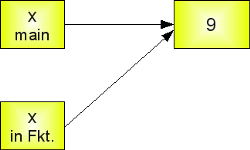
\includegraphics[width=0.7\linewidth,keepaspectratio]{boxes9}
\end{center}
        \end{column}
  \end{columns}
  
   % (Ref: https://www.python-course.eu/python3\_passing\_arguments.php)
   \end{frame}
   
 %%%%%%%%%%%%%%%%%%%%%%%%%%%%%%%%%%%%%%%%%%%%%%%%%%%%%%%%%%%%%%%%%%%%%%%%%%%%%%%%%%%
\begin{frame}[fragile]\frametitle{Python: ``Call by ??'' }
    \begin{itemize}
    \item As soon as a new value will be assigned to it, Python creates a separate local variable. 
    \item The caller's variable will not be changed this way: 
        \item After we have assigned the value 42 to x, x gets a new identity 41903752, i.e. a separate memory location from the global x. 
        \item  So, when we are back in the main scope x has still the original value 9. 
            \end{itemize}
  \begin{columns}[c]
    \begin{column}{0.5\linewidth}

            \begin{lstlisting}
            x = 9
def ref_demo(x):
    print("x=",x," id=",id(x))
    x=42
    print("x=",x," id=",id(x))
\end{lstlisting}

      \end{column}
    \begin{column}{0.4\linewidth}
    \begin{center}
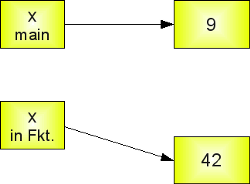
\includegraphics[width=0.7\linewidth,keepaspectratio]{boxes10}
\end{center}
        \end{column}
  \end{columns}
  
   % (Ref: https://www.python-course.eu/python3\_passing\_arguments.php)
   \end{frame}
   
    %%%%%%%%%%%%%%%%%%%%%%%%%%%%%%%%%%%%%%%%%%%%%%%%%%%%%%%%%%%%%%%%%%%%%%%%%%%%%%%%%%%
\begin{frame}[fragile]\frametitle{Python: ``Call by ??'' }

    \begin{itemize}
    \item This means that Python initially behaves like call-by-reference, but as soon as we are changing the value of such a variable, i.e. as soon as we assign a new object to it, Python "switches" to call-by-value. 
    \item This means that a local variable x will be created and the value of the global variable x will be copied into it. 
            \begin{lstlisting}
>>> x = 9
>>> id(x)
9251936
>>> ref_demo(x)
x= 9  id= 9251936
x= 42  id= 9252992
>>> id(x)
9251936
>>> 
\end{lstlisting}

            \end{itemize}
  
   (Ref: https://www.python-course.eu/python3\_passing\_arguments.php)
   \end{frame}
%
%
%
%
%
%%%%%%%%%%%%%%%%%%%%%%%%%%%%%%%%%%%%%%%%%%%%%%%%%%%%%%%%%%%%%%%%%%%%%%%%%%%%%%%%%%%%
%\begin{frame}[fragile]\frametitle{Modules}
%  The \texttt{import} statement reads a \texttt{.py} file, executes
%  it, and makes its contents available to the current program.
%\begin{lstlisting}
%>>> import re
%\end{lstlisting}
%\textbf{Modules are only read once}. Can call function multiple times.
%\begin{lstlisting}
%>>> import re
%match = re.compile(r'\d+', str)
%>>> import re
%>>> import re
%\end{lstlisting}
%
%\end{frame}
%
%%%%%%%%%%%%%%%%%%%%%%%%%%%%%%%%%%%%%%%%%%%%%%%%%%%%%%%%%%%%%%%%%%%%%%%%%%%%%%%%%%%%
%\begin{frame}[fragile]\frametitle{Modules}
%  Modules are \emph{namespaces:} 
%  Functions and variables defined in a module must be prefixed with the module name.
%
%\begin{lstlisting}
%>>> re.match(r'\d+',''Bob'')
%\end{lstlisting}
%To import definitions into the current namespace, use the
%  `\texttt{from $re$ import $match$}' form:
%\begin{lstlisting}
%>>> match(r'\d+',''Bob'')
%\end{lstlisting}
%To import ALL definitions into the current namespace, use the
%  `\texttt{from $re$ import $*$}' form:
%\end{frame}
%
%%%%%%%%%%%%%%%%%%%%%%%%%%%%%%%%%%%%%%%%%%%%%%%%%%%%%%%%%%%%%%%%%%%%%%%%%%%%%%%%%%%%
%\begin{frame}[fragile]\frametitle{The `return` statement}
%The result of a function evaluation is set by the \textit{return} statement.
%
%\begin{lstlisting}
%def double(x):
%  return x+x
%
%double(3) == 6
%\end{lstlisting}
%
%After executing \texttt{return} the control flow leaves the function.
%\begin{lstlisting}
%def double(x):
%  return x+x
%  # the following line is never exec'd
%  print('Hello')
%\end{lstlisting}
%
%
%\end{frame}
%
%%%%%%%%%%%%%%%%%%%%%%%%%%%%%%%%%%%%%%%%%%%%%%%%%%%%%%%%%%%%%%%%%%%%%%%%%%%%%%%%%%%%
%\begin{frame}[fragile]\frametitle{Globals}
%  \begin{itemize}
%  \item By default, assignment in a function or method creates local variables.
%  \item Reference (not assignment) to a variable, accesses a local variable if it has already been created, else accesses a global variable.
%  \item In order to assign a value to a global variable, declare the variable as global at the beginning of the function or method.
%  \item If in a function or method, you both reference and assign to a variable, then you must either:
%  \begin{itemize}
%  \item Assign to the variable first, or
%  \item Declare the variable as global
%    \end{itemize}
%  \end{itemize}
%\end{frame}

%%%%%%%%%%%%%%%%%%%%%%%%%%%%%%%%%%%%%%%%%%%%%%%%%%%%%%%%%%%%%%%%%%%%%%%%%%%%%%%%%%%%%
%%\begin{frame}[fragile]\frametitle{Type conversions}
%%  \begin{itemize}
%%  \item {\bf str($x$)} Converts the argument $x$ to a string; for numbers,
%%    the base 10 representation is used.
%%  \item {\bf int($x$)} Converts its argument $x$ (a number or a string) to an integer;
%%    if $x$ is a a floating-point literal, decimal digits are truncated.
%%  \item {\bf float($x$)} Converts its argument $x$ (a number or a string) to a
%%    floating-point number.
%%  \end{itemize}
%%
%%\end{frame}

%%%%%%%%%%%%%%%%%%%%%%%%%%%%%%%%%%%%%%%%%%%%%%%%%%%%%%%%%%%%%%%%%%%%%%%%%%%%%%%%%%%%%
%%\begin{frame}[fragile]  \frametitle{Special variables}
%%\begin{itemize}
%%\item Python relies on many special variables that can be accessed by your code.
%%\item One is the \lstinline{name} variables.
%%\item When a module is run, it contains the string \lstinline{main}.
%%\item When the module is imported, it contains the modules name.
%%\item You can add code that runs only when a module is called directly:\lstinline{if __name__ == __ main__: test()}
%%\end{itemize}
%%\end{frame}

% %%%%%%%%%%%%%%%%%%%%%%%%%%%%%%%%%%%%%%%%%%%%%%%%%%%%%%%%%%%%%%%%%%%%%%%%%%%%%%%%%%%
% \begin{frame}[fragile]\frametitle{lambda: anonymous functions}
% The following functions f and g do the same thing:

% \begin{lstlisting}
% def f(x): return x**2
% \end{lstlisting}

% \begin{lstlisting}
% g = lambda x: x**2
% \end{lstlisting}
% lambda functions can be place anywhere a function is expected
% without formal definition.

% \end{frame}

% %%%%%%%%%%%%%%%%%%%%%%%%%%%%%%%%%%%%%%%%%%%%%%%%%%%%%%%%%%%%%%%%%%%%%%%%%%%%%%%%%%%
% \begin{frame}[fragile]\frametitle{overloading}
% \begin{itemize}
% \item Python does not support method or function overloading. 
% \item You have to rely on the type() built-in function
% \end{itemize}
% \begin{lstlisting}
% def testtype(a):
	% if type(a) == types.FloatType:
		% print(``I got a float'')
	% elif type(A) == types.ComplexType:
		% print(``A complex number'')
	% else:
		% print(``something else'')
% \end{lstlisting}
% \end{frame}

% %%%%%%%%%%%%%%%%%%%%%%%%%%%%%%%%%%%%%%%%%%%%%%%%%%%%%%%%%%%%%%%%%%%%%%%%%%%%%%%%%%%
% \begin{frame}[fragile]\frametitle{Encrypt}
% \begin{lstlisting}
% plaintext    = list('ABCDEFGHIJKLMNOPQRSTUVWXYZ')
% encrytedtext = list('DEFGHIJKLMNOPQRSTUVWXYZABC')

% def message(text, plain, encryp):
    % dictionary = dict(zip(plain, encryp))
    % newmessage = ''
    % for char in text:
        % try:
            % newmessage += dictionary[char]
        % except:
            % newmessage += ' '
    % print(newmessage)

% message('SEND THE MATERIAL NOW')
% outputs: LTFR ZIT DQZTKOQS FGV
% \end{lstlisting}
% Write Decrypt function.
% \end{frame}

% %%%%%%%%%%%%%%%%%%%%%%%%%%%%%%%%%%%%%%%%%%%%%%%%%%%%%%%%%%%%%%%%%%%%%%%%%%%%%%%%%%%%%
% %%\begin{frame}[fragile]\frametitle{lambda}
% %%Use a lambda, as a convenience, when you need a function that both:
% %%\begin{itemize}
% %%\item is anonymous (does not need a name) and
% %%\item contains only an expression and no statements.
% %%\end{itemize}
% %%\begin{lstlisting}
% %%a = lambda x, y: (x * 3, y * 4, (x, y))
% %%a(3, 4)
% %%(9, 16, (3, 4))
% %%\end{lstlisting}
% %%\end{frame}

% %%%%%%%%%%%%%%%%%%%%%%%%%%%%%%%%%%%%%%%%%%%%%%%%%%%%%%%%%%%%%%%%%%%%%%%%%%%%%%%%%%%
% \begin{frame}[fragile]\frametitle{Iterators and generators}
% \begin{itemize}
% \item iterator: And iterator is something that satisfies the iterator protocol. Clue: If it's an iterator, you can use it in a  for:  statement.
% \item generator: A generator is a class or function that implements an iterator, i.e. that implements the iterator protocol.
% \item iterator protocol:  An object satisfies the iterator protocol if it does the following:
	% \begin{itemize}
	% \item It implements a  \lstinline|__iter__|  method, which returns an iterator object.
	% \item It implements a  \lstinline|next|  function, which returns the next item from the collection, sequence, stream, etc of items to be iterated over
	% \item It raises the  \lstinline|StopIteration|  exception when the items are exhausted and the  \lstinline|next()|  method is called.
	% \end{itemize}
% \end{itemize}

% \end{frame}

% %%%%%%%%%%%%%%%%%%%%%%%%%%%%%%%%%%%%%%%%%%%%%%%%%%%%%%%%%%%%%%%%%%%%%%%%%%%%%%%%%%%
% \begin{frame}[fragile]\frametitle{yield}
% \begin{itemize}
% \item yield: The  \lstinline{yield}  statement enables us to write functions that are generators. 
% \item The  \lstinline{yield}  statement returns a value. When the next item is requested and the iterator is ``resumed'', execution continues immediately after the  \lstinline{yield} statement.
% \item We can terminate the sequence generated by an iterator by using a  \lstinline{return} statement with no value.
% \item To resume a generator, use the generator's  \lstinline{next()}  or  \lstinline{send()}  methods. \lstinline{send()}  is like  \lstinline{next()} , but provides a value to the yield expression.
% \end{itemize}

% \begin{lstlisting}
% def list_tripler(somelist):
	% for item in somelist:
		% item *= 3
		% yield item

% it = list_tripler(alist)
	% for item in it:
		% print(item)
% \end{lstlisting}
% \end{frame}

% %%%%%%%%%%%%%%%%%%%%%%%%%%%%%%%%%%%%%%%%%%%%%%%%%%%%%%%%%%%%%%%%%%%%%%%%%%%%%%%%%%%
% \begin{frame}[fragile]\frametitle{Exercises}
% \begin{itemize}
% \item  Rewrite the grade program from the previous chapter using a function called computegrade that takes a score as its parameter and returns a grade as a
% string.
% \begin{lstlisting}
% Score Grade
% > 0.9 A
% > 0.8 B
% > 0.7 C
% > 0.6 D
% <= 0.6 F
% \end{lstlisting}
% \item Rewrite your pay computation with time-and-a-half for overtime and
% create a function called computepay which takes two parameters (hours and rate).
% \begin{lstlisting}
% Enter Hours: 45
% Enter Rate: 10
% Pay: 475.0
% \end{lstlisting}
% \end{itemize}


% \end{frame}

%%%%%%%%%%%%%%%%%%%%%%%%%%%%%%%%%%%%%%%%%%%%%%%%%%%%%%%%%%%%%%%%%%%%%%%%%%%%%%%%%%%
\begin{frame}[fragile]\frametitle{Recap (Functions)}
  \begin{itemize}
  \item Indentation is used to delimit blocks of code!
  \item Variables are just names, a reference to real object.
  \item \lstinline|def function(arg1, arg2, ...):| to define functions
  \item \lstinline|import filename| to use code from other files.
  % \item Modules are \textit{namespaces}.
  % \item Conversion between types with \lstinline|int(), float(), str()| functions.
  \item To get information on something: \lstinline|help(something)|
  \end{itemize}
\end{frame}